\documentclass[svgnames,11pt]{standalone}
\usepackage[utf8]{inputenc}
\usepackage[T1]{fontenc}
\usepackage{csquotes}
\usepackage[english]{babel}
\usepackage{xcolor}
\usepackage{charter}
\usepackage{amsmath}
\usepackage{amssymb}
\usepackage[np,autolanguage]{numprint}
\newcommand{\outqt}[1]{{\textcolor{DarkOrange}{#1}}}
\newcommand{\inqt}[1]{{\textcolor{Blue}{#1}}}
\usepackage{tikz}
\usetikzlibrary{arrows,automata,calc}
\usetikzlibrary{arrows.meta}
\usetikzlibrary{decorations.pathreplacing}
\usetikzlibrary{backgrounds,shapes}
\tikzset{%
  show curve controls/.style={
    postaction={
      decoration={
        show path construction,
        curveto code={
          \draw [blue] 
            (\tikzinputsegmentfirst) -- (\tikzinputsegmentsupporta)
            (\tikzinputsegmentlast) -- (\tikzinputsegmentsupportb);
          \fill [red, opacity=0.5] 
            (\tikzinputsegmentsupporta) circle [radius=.25ex]
            (\tikzinputsegmentsupportb) circle [radius=.25ex];
        }
      },
      decorate
}}}
\tikzstyle{vertex}=[draw,circle,black,inner sep=2pt]
\tikzstyle{edge}=[line width=1.3pt,color=Black]
\tikzstyle{rare}=[fill=black,text=white]
\tikzstyle{medium}=[fill=black!15!white]


\begin{document}
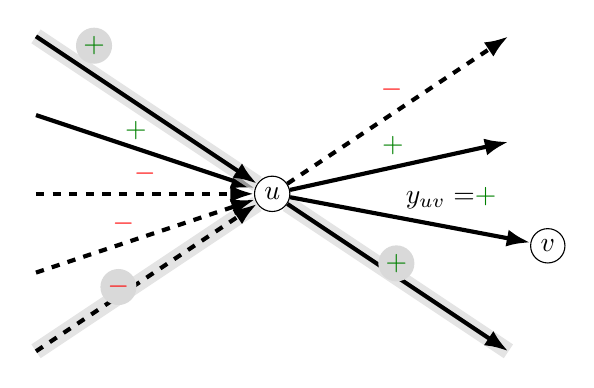
\begin{tikzpicture}[auto,vertex/.append style={minimum width=10mm}]
  \tikzset{>=latex}
  \tikzstyle{peers}=[draw,circle,black,inner sep=2pt,fill opacity=.0, text opacity=1]
  \tikzstyle{edge}=[line width=1.5pt,color=Black,-{Latex[length=3mm,width=1.0mm,angle'=40]}]
  \tikzstyle{trainEdge}=[line width=6pt,color=Black!15,opacity=.7]
  \tikzstyle{elabel}=[color=Black]
  \tikzstyle{posc}=[scale=1.0,text=Green]
  \tikzstyle{negc}=[scale=1.0,text=red]
  \tikzstyle{testset}=[opacity=1.0]
  \tikzstyle{revealed}=[circle,draw=none,fill=Black!15,inner sep=1pt,]

  \node[peers] (i) at (0,0) {$u$};
  \node[peers] (j) at (3.5,-0.66) {$v$};

  \draw[trainEdge] (i) --                                                           (3, -2);
  \draw[edge] (i) -- node [revealed,posc,xshift=-2mm,] {$\mathbf{+}$}                      (3, -2);

  \draw[testset,edge] (i) edge  node [posc,xshift=-2mm] {$\textcolor{Black}{y_{uv}=}+$} (j);
  \draw[testset,edge] (i) edge  node [posc,xshift=2mm] {$\mathbf{+}$}                    (3, 0.66);
  \draw[testset,edge, dashed] (i)   edge   node [negc,xshift=2mm] {$\mathbf{-}$} (3, 2);

  \draw[trainEdge] (-3, -2) --    (i);
  \draw[edge, dashed] (-3, -2) --   node [revealed,negc,yshift=-3mm,xshift=-5pt] {$\mathbf{-}$} (i);

  \draw[testset,edge, dashed] (-3, -1) --   node [negc,yshift=-1mm] {$\mathbf{-}$} (i);
  \draw[testset,edge, dashed] (-3, 0)  --  node [negc] {$\mathbf{-}$} (i);
  \draw[testset,edge,]                (-3, 1) --   node [posc,xshift=-4mm] {$\mathbf{+}$} (i);

  \draw[trainEdge,]           (-3, 2) --   (i);
  \draw[edge,]                (-3, 2) --   node [revealed,posc,above,pos=0.2,xshift=5pt] {$\mathbf{+}$} (i);

  % \node[fill=white!90!DarkOrange,fill opacity=.9,text opacity=1,rounded corners,inner sep=2pt] at (1,-1.5) {$tr(i)=\frac{1}{4}$};
  % \node[fill=white!90!Blue,fill opacity=.5,text opacity=1,rounded corners,inner sep=2pt] at (-1.0,1.7) {$un(i)=\frac{3}{5}$};
\end{tikzpicture}
\end{document}
